%===============================================================================
% LaTeX sjabloon voor de bachelorproef toegepaste informatica aan HOGENT
% Meer info op https://github.com/HoGentTIN/bachproef-latex-sjabloon
%===============================================================================

\documentclass{bachproef-tin}

\usepackage{hogent-thesis-titlepage} % Titelpagina conform aan HOGENT huisstijl
\usepackage{lipsum}
\usepackage{biblatex}

\bibliography{bachproef-tin.bib}{}

%%---------- Documenteigenschappen ---------------------------------------------
% TODO: Vul dit aan met je eigen info:

% De titel van het rapport/bachelorproef
\title{Microservice integration patterns on SAP order-to-cash process.}

% Je eigen naam
\author{Lyva Van Damme}

% De naam van je promotor (lector van de opleiding)
\promotor{Karin Samyn}

% De naam van je co-promotor. Als je promotor ook je opdrachtgever is en je
% dus ook inhoudelijk begeleidt (en enkel dan!), mag je dit leeg laten.
\copromotor{Nicolas Pauwelyn}

% Indien je bachelorproef in opdracht van/in samenwerking met een bedrijf of
% externe organisatie geschreven is, geef je hier de naam. Zoniet laat je dit
% zoals het is.
\instelling{HoGent}

% Academiejaar
\academiejaar{2018-2019}

% Examenperiode
%  - 1e semester = 1e examenperiode => 1
%  - 2e semester = 2e examenperiode => 2
%  - tweede zit  = 3e examenperiode => 3
\examenperiode{2}

%===============================================================================
% Inhoud document
%===============================================================================

\begin{document}

%---------- Taalselectie -------------------------------------------------------
% Als je je bachelorproef in het Engels schrijft, haal dan onderstaande regel
% uit commentaar. Let op: de tekst op de voorkaft blijft in het Nederlands, en
% dat is ook de bedoeling!

%\selectlanguage{english}

%---------- Titelblad ----------------------------------------------------------
\inserttitlepage

%---------- Samenvatting, voorwoord --------------------------------------------
\usechapterimagefalse
%%=============================================================================
%% Voorwoord
%%=============================================================================

\chapter*{\IfLanguageName{dutch}{Woord vooraf}{Preface}}
\label{ch:voorwoord}

%% TODO:
%% Het voorwoord is het enige deel van de bachelorproef waar je vanuit je
%% eigen standpunt (``ik-vorm'') mag schrijven. Je kan hier bv. motiveren
%% waarom jij het onderwerp wil bespreken.
%% Vergeet ook niet te bedanken wie je geholpen/gesteund/... heeft
Deze bachelorproef werd geschreven voor het behalen van het bachelordiploma Toegepaste Informatica. Eerst was het niet gemakkelijk om een onderwerp te vinden. Ik wist niet goed waar ik het over wou hebben. Ik zou daarvoor graag mijn stagebedrijf, Delaware, voor het voorstellen van een onderwerp. Dankzij hun ben ik op een onderwerp gekomen waar ik interesse in had. 
Ik zou ook graag mijn ouders bedanken voor de steun die zij mij gaven. Voor hun geduld bij de stressvolle situaties. Ook wil ik mijn broer en zus bedanken voor hun hulp.

%%=============================================================================
%% Samenvatting
%%=============================================================================

% TODO: De "abstract" of samenvatting is een kernachtige (~ 1 blz. voor een
% thesis) synthese van het document.
%
% Deze aspecten moeten zeker aan bod komen:
% - Context: waarom is dit werk belangrijk?
% - Nood: waarom moest dit onderzocht worden?
% - Taak: wat heb je precies gedaan?
% - Object: wat staat in dit document geschreven?
% - Resultaat: wat was het resultaat?
% - Conclusie: wat is/zijn de belangrijkste conclusie(s)?
% - Perspectief: blijven er nog vragen open die in de toekomst nog kunnen
%    onderzocht worden? Wat is een mogelijk vervolg voor jouw onderzoek?
%
% LET OP! Een samenvatting is GEEN voorwoord!

%%---------- Nederlandse samenvatting -----------------------------------------
%
% TODO: Als je je bachelorproef in het Engels schrijft, moet je eerst een
% Nederlandse samenvatting invoegen. Haal daarvoor onderstaande code uit
% commentaar.
% Wie zijn bachelorproef in het Nederlands schrijft, kan dit negeren, de inhoud
% wordt niet in het document ingevoegd.

\IfLanguageName{english}{%
\selectlanguage{dutch}
\chapter*{Samenvatting}

\selectlanguage{english}
}{}

%%---------- Samenvatting -----------------------------------------------------
% De samenvatting in de hoofdtaal van het document

\chapter*{\IfLanguageName{dutch}{Samenvatting}{Abstract}}

% CONTEXT

% NOOD
Dit onderwerp werd gegeven door delaware. Om te onderzoeken hoe microservices een invloed kan hebben op het order-to-cash proces binnen SAP. 

% TAAK
Dit onderzoek kent een verdiepende structuur. Waar in de start uitleg wordt gegeven omtrent microservices, kent het vervolg een vergelijking tussen verschillende onderdelen. Enkele voorbeelden hiervan zijn authenticatie en authorisatie. Deze scriptie sluit af met opkomende ideologieën en de bescherming van microservices.

% OBJECT

% RESULTAAT

% CONCLUSIE

% PERSPECTIEF
Er zullen zeker vragen en aanvullingen komen in de toekomst. Dit is een evoluerende technologie en er zullen betere oplossingen komen voor onderdelen.

%---------- Inhoudstafel -------------------------------------------------------
\pagestyle{empty} % Geen hoofding
\tableofcontents  % Voeg de inhoudstafel toe
\cleardoublepage  % Zorg dat volgende hoofstuk op een oneven pagina begint
\pagestyle{fancy} % Zet hoofding opnieuw aan

%---------- Lijst figuren, afkortingen, ... ------------------------------------

% Indien gewenst kan je hier een lijst van figuren/tabellen opgeven. Geef in
% dat geval je figuren/tabellen altijd een korte beschrijving:
%
%  \caption[korte beschrijving]{uitgebreide beschrijving}
%
% De korte beschrijving wordt gebruikt voor deze lijst, de uitgebreide staat bij
% de figuur of tabel zelf.

\listoffigures
\listoftables

% Als je een lijst van afkortingen of termen wil toevoegen, dan hoort die
% hier thuis. Gebruik bijvoorbeeld de ``glossaries'' package.
% https://www.overleaf.com/learn/latex/Glossaries

%---------- Kern ---------------------------------------------------------------

% De eerste hoofdstukken van een bachelorproef zijn meestal een inleiding op
% het onderwerp, literatuurstudie en verantwoording methodologie.
% Aarzel niet om een meer beschrijvende titel aan deze hoofstukken te geven of
% om bijvoorbeeld de inleiding en/of stand van zaken over meerdere hoofdstukken
% te verspreiden!

%%=============================================================================
%% Inleiding
%%=============================================================================

\chapter{\IfLanguageName{dutch}{Inleiding}{Introduction}}
\label{ch:inleiding}

De inleiding moet de lezer net genoeg informatie verschaffen om het onderwerp te begrijpen en in te zien waarom de onderzoeksvraag de moeite waard is om te onderzoeken. In de inleiding ga je literatuurverwijzingen beperken, zodat de tekst vlot leesbaar blijft. Je kan de inleiding verder onderverdelen in secties als dit de tekst verduidelijkt. Zaken die aan bod kunnen komen in de inleiding~\autocite{Pollefliet2011}:

\begin{itemize}
  \item context, achtergrond
  \item afbakenen van het onderwerp
  \item verantwoording van het onderwerp, methodologie
  \item probleemstelling
  \item onderzoeksdoelstelling
  \item onderzoeksvraag
  \item \ldots
\end{itemize}

\section{\IfLanguageName{dutch}{Probleemstelling}{Problem Statement}}
\label{sec:probleemstelling}
Dit onderzoek werd voorgesteld door Delaware. Zij hadden dit onderwerp voorgesteld. De doelgroep is dus Delaware.

Uit je probleemstelling moet duidelijk zijn dat je onderzoek een meerwaarde heeft voor een concrete doelgroep. De doelgroep moet goed gedefinieerd en afgelijnd zijn. Doelgroepen als ``bedrijven,'' ``KMO's,'' systeembeheerders, enz.~zijn nog te vaag. Als je een lijstje kan maken van de personen/organisaties die een meerwaarde zullen vinden in deze bachelorproef (dit is eigenlijk je steekproefkader), dan is dat een indicatie dat de doelgroep goed gedefinieerd is. Dit kan een enkel bedrijf zijn of zelfs één persoon (je co-promotor/opdrachtgever).

\section{\IfLanguageName{dutch}{Onderzoeksvraag}{Research question}}
\label{sec:onderzoeksvraag}
Hoe microserivce integration patterns een order-to-cash proces in SAP kan beïnvloeden? Dit is de algemene onderzoeksvraag. Om het concreter te maken gaan we eerst gaan een duidelijk beeld tekenen van 'Wat zijn microservices?'. Daarnaast gaan we kijken wat de grote technologische bedrijven, zoals Facebook, Amazon, Netflix, gedaan hebben bij het overschakelen naar microservices. Daar kan men al een antwoord op geven. Maar eerst willen we elk deeltje van de onderzoeksvraag goed uitleggen. Ook zal er een deel van deze bachelorproef gaan over 'Hoe een order-to-cash proces er in SAP uitziet.'. Het eerst uitleggen van de twee grootste onderdelen van deze bachelorproef, moet een duidelijker beeld geven over de algemene onderzoeksvraag. Dan als de twee onderdelen grondig uitgelegd en onderzocht zijn, gaat er gekeken worden hoe de microservices een invloed kan hebben op een order-to-cash proces binnen SAP. Wat er zal moeten aangepast worden om de microservices te kunnen gebruiken. Er zal gekeken worden naar de business requirements van een order-to-cash proces. Op welke manier zullen de microservices met elkaar communiceren? is ook een van de belangrijke vraag die zal beantwoord worden. Dit zal een theoretische studie zijn. Er zal geen proof of concept komen wegens tijdsgebrek. 

\section{\IfLanguageName{dutch}{Onderzoeksdoelstelling}{Research objective}}
\label{sec:onderzoeksdoelstelling}
Het resultaat van deze proef zal af hangen van hoe de vergelijkende studie zal gaan. De criteria voor succes zijn opgesteld vanuit de business. Het slagen van deze proef is afhankelijk van de business requirements. Er zal een theoretische studie plaatsvinden. Deze zal gaan over wat microservices zijn, wat een order-to-cash proces in SAP inhoudt en welke invloed microservices zullen hebben op het proces. Ook zal onderzocht worden wat er verandert.

\section{\IfLanguageName{dutch}{Opzet van deze bachelorproef}{Structure of this bachelor thesis}}
\label{sec:opzet-bachelorproef}

% Het is gebruikelijk aan het einde van de inleiding een overzicht te
% geven van de opbouw van de rest van de tekst. Deze sectie bevat al een aanzet
% die je kan aanvullen/aanpassen in functie van je eigen tekst.

De rest van deze bachelorproef is als volgt opgebouwd:

In Hoofdstuk~\ref{ch:stand-van-zaken} wordt een overzicht gegeven van de stand van zaken binnen het onderzoeksdomein, op basis van een literatuurstudie. Hierin zal er meer uitleg gegeven worden over microservices en het order-to-cash proces binnen SAP.

In Hoofdstuk~\ref{ch:methodologie} wordt de methodologie toegelicht en worden de gebruikte onderzoekstechnieken besproken om een antwoord te kunnen formuleren op de onderzoeksvragen. Hier zal het onderzoek worden uitgevoerd over hoe microservices het order-to-cash proces zullen beïnvloeden.

% TODO: Vul hier aan voor je eigen hoofstukken, één of twee zinnen per hoofdstuk

In Hoofdstuk~\ref{ch:conclusie}, tenslotte, wordt de conclusie gegeven en een antwoord geformuleerd op de onderzoeksvragen. Daarbij wordt ook een aanzet gegeven voor toekomstig onderzoek binnen dit domein.
\chapter{\IfLanguageName{dutch}{Stand van zaken}{State of the art}}
\label{ch:stand-van-zaken}

% Tip: Begin elk hoofdstuk met een paragraaf inleiding die beschrijft hoe
% dit hoofdstuk past binnen het geheel van de bachelorproef. Geef in het
% bijzonder aan wat de link is met het vorige en volgende hoofdstuk.

% Pas na deze inleidende paragraaf komt de eerste sectiehoofding.

Dit hoofdstuk bevat je literatuurstudie. De inhoud gaat verder op de inleiding, maar zal het onderwerp van de bachelorproef *diepgaand* uitspitten. De bedoeling is dat de lezer na lezing van dit hoofdstuk helemaal op de hoogte is van de huidige stand van zaken (state-of-the-art) in het onderzoeksdomein. Iemand die niet vertrouwd is met het onderwerp, weet nu voldoende om de rest van het verhaal te kunnen volgen, zonder dat die er nog andere informatie moet over opzoeken \autocite{Pollefliet2011}.

\section{Microservices}
\subsection{Definitie}
Hier zal de definitie komen van microservices
\subsection{Het belang van microservices}
Hier zal de 'nood' aan microservices uitgeschreven worden.
\subsection{Algemene aanpak om microservices te implementeren}
Hoe microservices in het algemeen worden geimplementeerd.
\subsection{De voordelen en nadelen van microserivces}
Wat is er goed en slecht aan microserivces.
\subsection{Voorbeelden}
Hier komen voorbeelden van grote techno bedrijven.

\section{Order-to-cash proces in SAP}
\subsection{Definite}
De definitie van een order-to-cash proces.
\subsection{Technologie}
\subsubsection{Onderdelen van een order-to-cash proces}
\subsubsection{Wat biedt SAP zelf aan voor microservices}
\subsection{Een order-to-cash proces vanuit de business}
\subsection{Het proces afstemmen met de business}

\section{Requirements van de business}
Je verwijst bij elke bewering die je doet, vakterm die je introduceert, enz. naar je bronnen. In \LaTeX{} kan dat met het commando \texttt{$\backslash${textcite\{\}}} of \texttt{$\backslash${autocite\{\}}}. Als argument van het commando geef je de ``sleutel'' van een ``record'' in een bibliografische databank in het Bib\LaTeX{}-formaat (een tekstbestand). Als je expliciet naar de auteur verwijst in de zin, gebruik je \texttt{$\backslash${}textcite\{\}}.
Soms wil je de auteur niet expliciet vernoemen, dan gebruik je \texttt{$\backslash${}autocite\{\}}. In de volgende paragraaf een voorbeeld van elk.

\textcite{Knuth1998} schreef een van de standaardwerken over sorteer- en zoekalgoritmen. Experten zijn het erover eens dat cloud computing een interessante opportuniteit vormen, zowel voor gebruikers als voor dienstverleners op vlak van informatietechnologie~\autocite{Creeger2009}.

\lipsum[7-20]

%%=============================================================================
%% Methodologie
%%=============================================================================

\chapter{\IfLanguageName{dutch}{Methodologie}{Methodology}}
\label{ch:methodologie}

In dit hoofdstuk zal er een schets gemaakt worden van het OTC proces met een microservice architectuur. 

Eerst worden er enkele termen uitgelegd. Dan worden alle microservices binnen het OTC proces uitgelgd. Wat ze precies doen en tot welk onderdeel, van het OTC proces, ze behoren. Hierna wordt de communicatiemethode tussen de verschillende microservices uitgelegd. Als voorlaatste wordt de databank structuur uitgetekend. Als laatste wordt de complete architectuur uitgelegd. Onder de complete architectuur worden volgende punten aangehaald:
\begin{itemize}
	\item De communicatie tussen de onderdelen van het OTC proces. Hier wordt aan de hand van een schema uitgelegd hoe de communicatie gebeurt tussen de onderdelen.
	\item De architectuur. Dit deel bevat een schema, waar duidelijk op wordt welk onderdeel welke microservices aanspreekt. Per onderdeel wordt ook uitgelegd waarom deze microservices worden aangesproken.
	\item Als laatste worden de API gateway, logging, authenticatie en authorisatie toegevoegd.
\end{itemize}

\section{Uitleg termen}
In tabel 3.1 zijn termen terug te vinden die in dit hoofdstuk regelmatig zullen voorkomen.

\begin{table}[]
	\resizebox{\textwidth}{!}{%
		\begin{tabular}{|l|p{15cm}|}
			\hline 
			Queue & Een wachtrij waar berichten op geplaatst worden. Het bericht op de queue kan maar één keer gelezen worden. \\ \hline
			Consumption & De term om een bericht van de queue te lezen. \\ \hline
			Acknowledgement & Het verwijderen van een bericht op de queue. \\ \hline
			Overhead &  Als er teveel data aanwezig is op de queue dan spreekt men van overhead. Dit kan er voor zorgen dat de queue geen berichten meer ontvangt. \\ \hline
			Datastore &  Een datastore is een kleinere versie van een databank. Er kunnen files in opgeslaan worden. \\ \hline
		\end{tabular}%
	}
	\caption{Termen die vaker voorkomen in dit hoofdstuk.}
\end{table}

\section{De verschillende microservices binnen het OTC proces}
De microservices die logging, authenticatie, authorisatie en bescherming omvatten, zullen niet uitgelegd worden.
Voor elk van volgende microservices gaan we volgende vragen beantwoorden:
\begin{itemize}
	\item Wat kunnen ze?
	\item Hoe ziet de databank eruit?
	\item Welk deeltje van de databank spreken ze aan?
	\item Waar kunnen ze gebruikt worden?
	\item Waarom werd hiervan een microservice gemaakt?
\end{itemize}

\subsection{Klantengegevens ophalen}
Deze microservice gaat ervoor zorgen dat de klantengegevens uit de databank worden gehaald. Het zal de databank aanspreken en vragen om de data van een specifieke klant. 
Hoe het schema van de databank er uit ziet, is terug te vinden in het vorige deel. 
Deze microservice wordt gebruikt in meerdere delen van het order-to-cash proces. Een van de voordelen van microservices is de schaalbaarheid. Omdat de requirement meermaals zal voorkomen in het proces, is het voordeliger om de microservice te dupliceren en te hergebruiken. 
Deze microservice komt voor in volgende onderdelen:
\begin{itemize}
	\item Order management
	\item Credit management
	\item Klant management
	\item Facturatie
	\item Accounts receivables
\end{itemize}

\subsection{Orders plaatsen, ophalen en verwijderen}
Een belangrijk onderdeel is het plaatsen, ophalen en verwijderen van orders. Deze microservice heeft verschillende verantwoordelijkheden en rechten op de databank. 
Deze microservice zal gebruikt worden in volgende onderdelen:
\begin{itemize}
	\item Order management
	\item Order fullfilment
	\item Facturatie
\end{itemize}

\subsection{Producten ophalen en het aantal in voorraad veranderen}
In het order-to-cash proces worden er geen producten toegevoegd aan de lijst dus moet dit niet in een microservice gestoken worden. Het aantal van de voorraad moet worden aangepast wanneer er een product uit de rekken wordt gehaald en bij een bestelling wordt geplaatst. Het ophalen van producten is vooral voor het werk achter de schermen. Het ophalen van een product omvat vooral de verkoopprijs ophalen om die dan te gebruiken in de orderlijn. 
Deze microservice zal gebruikt worden in volgende onderdelen:
\begin{itemize}
	\item Order management
	\item order fullfilment
\end{itemize}

\subsection{Facturatie maken en ophalen}
Het begin van het einde in een order-to-cash proces. Facturen maken en ophalen zijn van groot belang bij een order-to-cash proces. Het zorgt er voor dat mensen geld gaan betalen voor hun order. Een factuur moet overeenstemmen met wat geleverd is. Het is van groot belang dat achter kan gekeken worden of de factuur klopt met de order. Het maken van de factuur gebeurt aan de hand van het order. 
Deze microservice komt voor in het onderdeel facturatie.

\subsection{Shipment documentatie opstellen}
Het shipment document wordt gegenereerd afhankelijk van het order. Er wordt gekeken naar het ordernummer en dan wordt er gekeken naar het klantnummer. Hierna wordt dan de microservice om klantgegevens op te halen aangesproken om de gegevens van de specifieke klant op te halen. Dit wordt enkel gebruikt binnen het onderdeel verzending.

\subsection{Aanmaning opmaken en verwijderen}
Het opmaken en verwijderen van aanmaningen gebeurt enkel wanneer een wanbetaler is. Het proces zou niet vaak mogen voorkomen. 

\subsection{Berichten plaatsen op de queue}
Berichten plaatsen op de queue met de correcte gegevens. Deze microservice zorgt daarvoor. Hiervan wordt een microservice gemaakt omdat dit in elke stap voorkomt. Het is dan eenvoudiger om er een microservice van te maken, zodat elk onderdeel op een uniforme manier het bericht plaatst. 
Deze microservice komt voor in elk onderdeel van het proces.

\subsection{Berichten ophalen van de queue} 
Elk onderdeel moet berichten van zijn queue kunnen halen. Door het meermaals voorkomen van deze taak, wordt er een microservice van gemaakt. Het ophalen van berichten gebeurt dan op een uniforme manier. 
Deze microservice komt voor in elk onderdeel van het proces.

\section{Communicatie methode tussen microservices}
Microservices moeten met elkaar kunnen communiceren. De manier wordt voorgesteld in figuur 3.1. 
Klant 66 plaats een order met vier verschillende producten. Het ordernummer is 23. De volledige bestelling komt binnen in het systeem en wordt op de queue van ordermanagement geplaatst. Het order wordt van de queue gehaald aan de hand van consumption en acknowledgement. Ordermanagement verwerkt de binnengekomen order. Dan wordt het klantnummer en ordernummer op de queue van creditmanagement geplaatst. Creditmanagement haalt het bericht van de queue. Dan wordt er gekeken naar het betaalgedrag van de klant. Is het een wanbetaler of betaalt de klant altijd correct. Staat de klant gekend voor wanbetalen, dan wordt er geen goedkeuring gegeven om het order te plaatsen. Bij een corect betaalgedrag, krijgt het order goedkeuring om geplaatst te worden. Dan wordt het ordernummer doorgestuurd naar het volgende deel van het proces. 
Dus volgende queue's zouden moeten bestaan:
\begin{itemize}
	\item QorderMan is een queue voor order management: Het plaatsen van een order.
	\item QcreditMan is een queue voor credit management: Om te controleren of een klant wel een order mag plaatsen.
	\item QorderFul is een queue voor order fulfilment: Het ophalen van de order in het magazijn.
	\item QorderShip is een queue voor order shipment: Het plannen van de route en welke goederen op welke vrachtwagen moeten geladen worden.
	\item Qfact is een queue voor de facturatie.
	\item QaccountsRec is een queue voor accounts receivable: De betaling van de factuur nagaan en tijdig aanmaningen sturen. 
\end{itemize}

Niet alle data wordt volledig naar de queue gestuurd enkel de belangrijke data. Zoals bijvoorbeeld het nummer van de klant die een order plaatste. Het ordernummer en klantnummer worden naar creditmanagement doorgestuurd. Bij creditmanangement wordt er dan aan de hand van het klantnummer de gegevens opgehaald en dan zo nagegaan of die klant wel een order mag plaatsen. Het ordernummer werd meegestuurd om zeker te zijn dat de correcte order goed- of afgekeurd wordt. Zo blijft de overhead op de queue minimaal. Om meer gegevens op te halen, moet de databank aangesproken worden. De gehele structuur van de databank wordt beschreven in het volgende gedeelte.

\section{De databank structuur}
Onderliggend is één grote databank waar alle masterdata in terug te vinden is. Hier is de enige plaats waar een single point-of-failure terug te vinden is. Naast de grote databank, heeft elke microservice zijn datastore. Bij een verandering in een datastore, wordt deze aangebracht in de algemene databank. Eens de databank het record heeft toegevoegd of aangepast, stuurt hij een bericht naar elke datastore zijn queue om te melden dat er een verandering gebeurt is. 
\begin{figure}[h]
	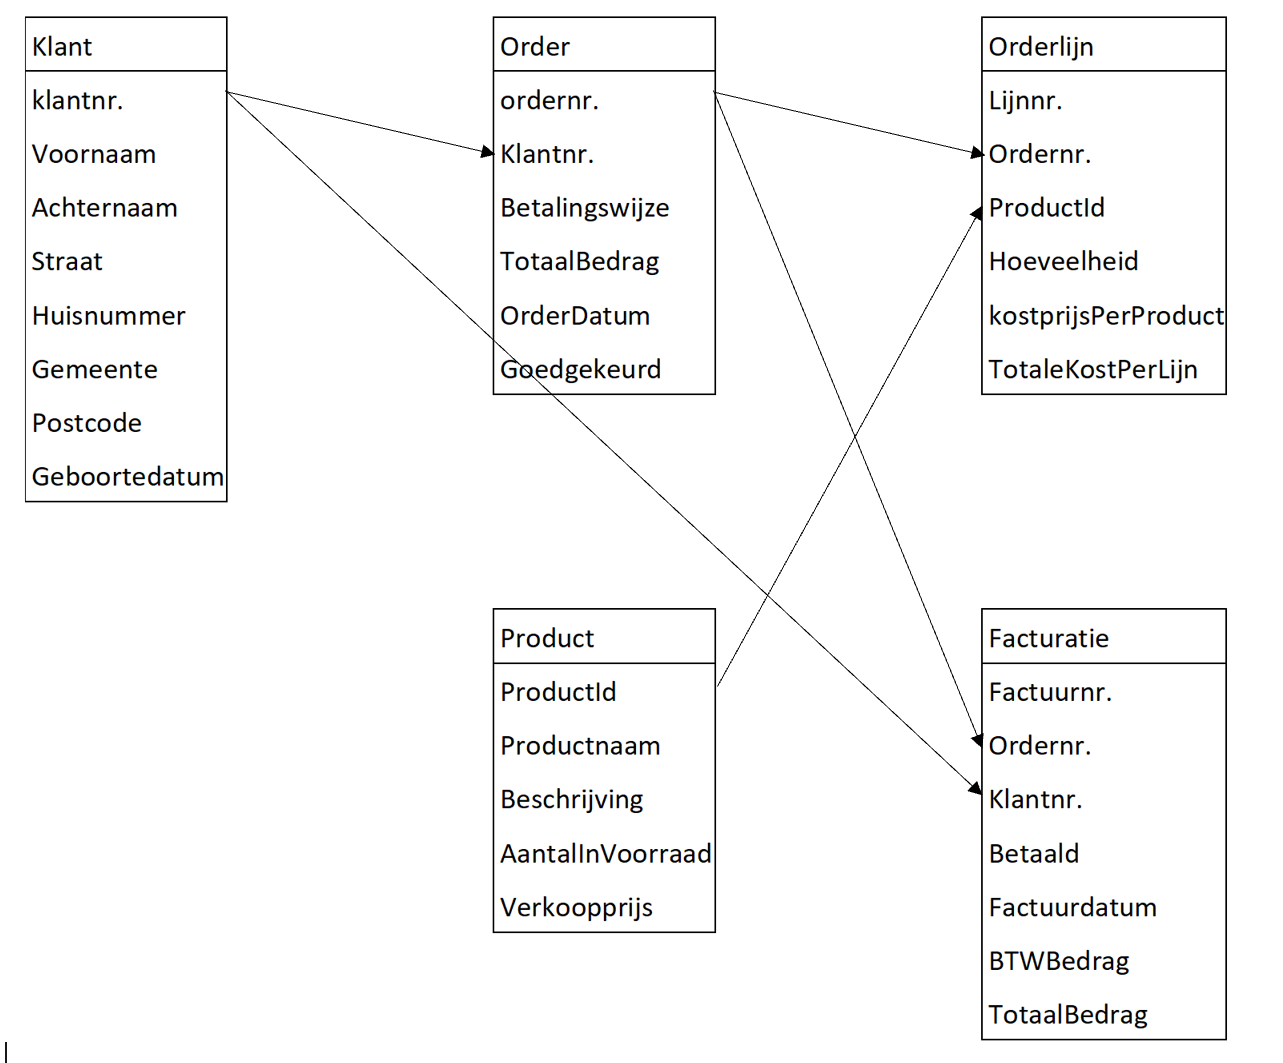
\includegraphics[width=15cm]{databank.png}
	\caption{De databank structuur.}
	\centering
\end{figure}

Een order weet wie zijn klant is. Credit management kan de eigenschap bij het order veranderen van 'goedgekeurd' naar 'niet goedgekeurd'. Van elk order wordt een orderlijn bijgehouden. Zodat er geweten is wat er op de order staat. Op elk orderlijn staat er een product of service. Van het product moet er een beschrijving en verkoopprijs zijn. Het aantal in voorraad is gekend omdat bij het order fullfilment moet de voorraad aangepast worden van het specifieke product. Een order en de klant zijn gekend op de facturatie. Zo kan er nagegaan worden of de factuur overeenkomt met wat er op het order staat. De klant zijn gegevens moeten gekend zijn om naar het juiste adres te factureren.

\section{De complete architectuur opbouwen}
Op figuur 3.3 is te zien hoe het proces in elkaar ziet. Door de microservice architectuur toe te passen op het order-to-cash proces verandert er niks aan de volgorde van het proces of het doel van het proces. De manier waarop gegevens worden opgehaald, verandert wel. 

\subsection{De communicatie tussen de onderdelen van het OTC proces}

\begin{figure}[h]
	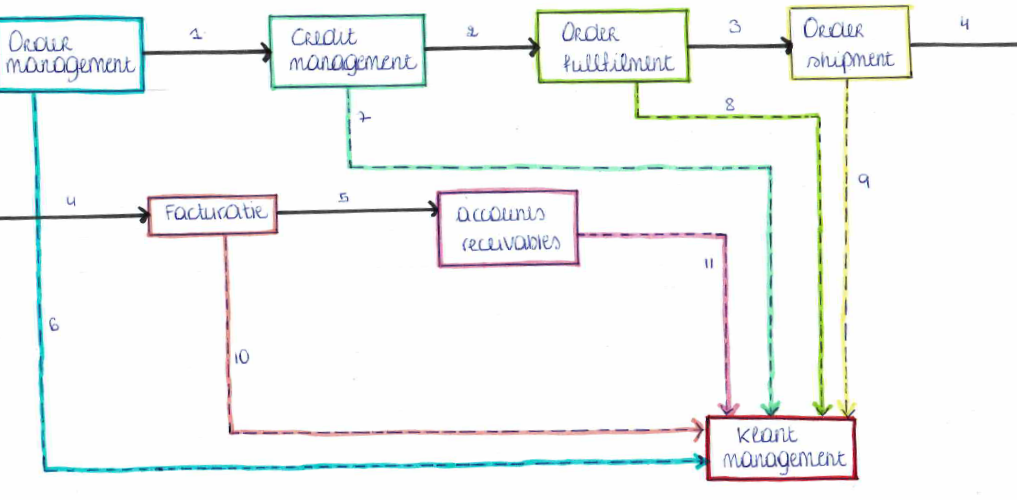
\includegraphics[width=15cm]{schema_communicatie.png}
	\caption{De communicatie tussen de verschillende onderdelen van het order-to-cash proces.}
	\centering
\end{figure}
Op figuur 3.3 is het communicatie patroon zichtbaar.
Voordat het proces van start kan gaan, moet een klant een order plaatsen. Een order bevat een aantal producten. Eens de klant een order geplaatst heeft dan is er een ordernummer gekend. De klant staat bekend in het systeem met een klantnummer. Dat zijn twee belangrijke gegevens die veel gebruikt zullen worden.
Meer uitleg over wat elk onderdeel doet, bevindt zich in het volgende hoofdstuk.
De nummers van de opsomming komen overeen met die op afbeelding 3.2.
\begin{enumerate}
	\item De communicatie tussen ordermanagement en creditmanagement. Er is een order geplaatst door klant 66. Ordermanagement zorgt ervoor dat het order in de databank geraakt. Eens de taak van ordermanagement gedaan is, plaatst die het klantnummmer en het ordernummer op de queue van creditmanagement. Dan is zijn taak gedaan. Ordermanagement houdt zich niet bezig met wat er gebeurt nadat hij het bericht geplaatst heeft.
	\item De communicatie tussen creditmanagement en order fullfilment. Creditmanagement heeft het ordernummer en klantnummer van ordermanagement gekregen. Het bericht wordt van de queue gehaald. Creditmanagement gaat dan aan de hand van de klantgegevens beslissen of de klant het order mag plaatsen of niet. Is het order goedgekeurd dan wordt het ordernummer op de queue van order fullfilment gezet. Er moet niet worden teruggekeerd naar order management. Credit management heeft de rechten om het veld goedgekeurd aan te passen. De taak van creditmanagement is nu afgerond.
	\item De communicatie tussen order fullfilment en order shipment. Order fullfilment heeft het ordernummer doorgekregen van credit management. Order fullfilment geeft het ordernummer door aan order shipment eens zijn taak gedaan is. 
	\item De communicatie tussen order shipment en de facturatie. Het ordernummer werd op de queue van order shipment geplaatst. Eens alles opgemaakt is bij order shipment, wordt het ordernummer doorgestuurd naar de facturatie. De taak van order shipment is afgerond.
	\item De communicatie tussen facturatie en accounts receivables. De facturatie kreeg een bericht van order shipment om de factuur op te maken voor het order met des betreffende ordernummer. Is de taak van facturatie afgerond dan wordt de factuurnummer doorgestuurd naa accounts receivables. Zodat de betaling verder kan worden opgevolgd.
	\item Ordermanagement plaatst het ordernummer op de queue van klant management. Klant management stuurt een bevestiging naar de klant van het goed ontvangen van zijn/haar order. En laat weten dat er eerst een controle komt op het betaalbedrag van de klant.
	\item Creditmanagement plaatst het ordernummer en de status van goedgekeurd of afgekeurd op de queue. Dan wordt er een bericht verzonden naar de klant. Het bericht bevat de info of de klant zijn order is goedgekeurd of afgekeurd.
	\item Order fullfilment plaatst een bericht op de queue om te laten weten dat het order gemaakt is. Dat de goederen uit het magazijn zijn opgehaald en klaar gemaakt worden voor verzending.
	\item Order shipment plaatst een bericht op de queue wanneer de goederen klaar zijn voor vertrek. Klant management zorgt er dan voor dat het bericht tot bij de klant geraakt.
	\item Facturatie plaatst een bericht op de queue van klant management om ervoor te zorgen dat de factuur tot bij de klant geraakt.
	\item Accounts receivables plaatst een bericht op de queue van klant management als er aanmaningen moeten worden gestuurd.
\end{enumerate}

\subsection{De architectuur}
In volgende tabel, zijn er letters en bijhorende microservices terug te vinden. Deze worden gebruikt bij het uitleggen van de architectuur.
\begin{table}[]
	\resizebox{\textwidth}{!}{%
		\begin{tabular}{|l|p{15cm}|}
			\hline 
			A & Klantgegevens ophalen \\ \hline
			B & Orders plaatsen, ophalen en verwijderen \\ \hline
			C & Producten ophalen en het aantal van voorraad aanpassen \\ \hline
			D & Shipment documenten opstellen \\ \hline
			E & Facturatie maken en ophalen \\ \hline
			F & Aanmaning opmaken en verwijderen \\ \hline
			G & Bericht plaatsen op de queue \\ \hline
			H & Bericht ophalen van de queue \\ \hline
		\end{tabular}%
	}
	\caption{Legende die gebruikt wordt in de afbeeldingen.}
\end{table}

In tabel 3.2 is de legende terug te vinden die gebruikt wordt bij het uitleggen van elk onderdeel apart.
In figuur 3.3 is te zien hoe het volledige proces communiceert met de verschillende microservices. Elk onderdeel van het proces is een microservice op zich. Een microservice die meerdere microservices aanspreekt om goed te functioneren.
\begin{figure}[h]
	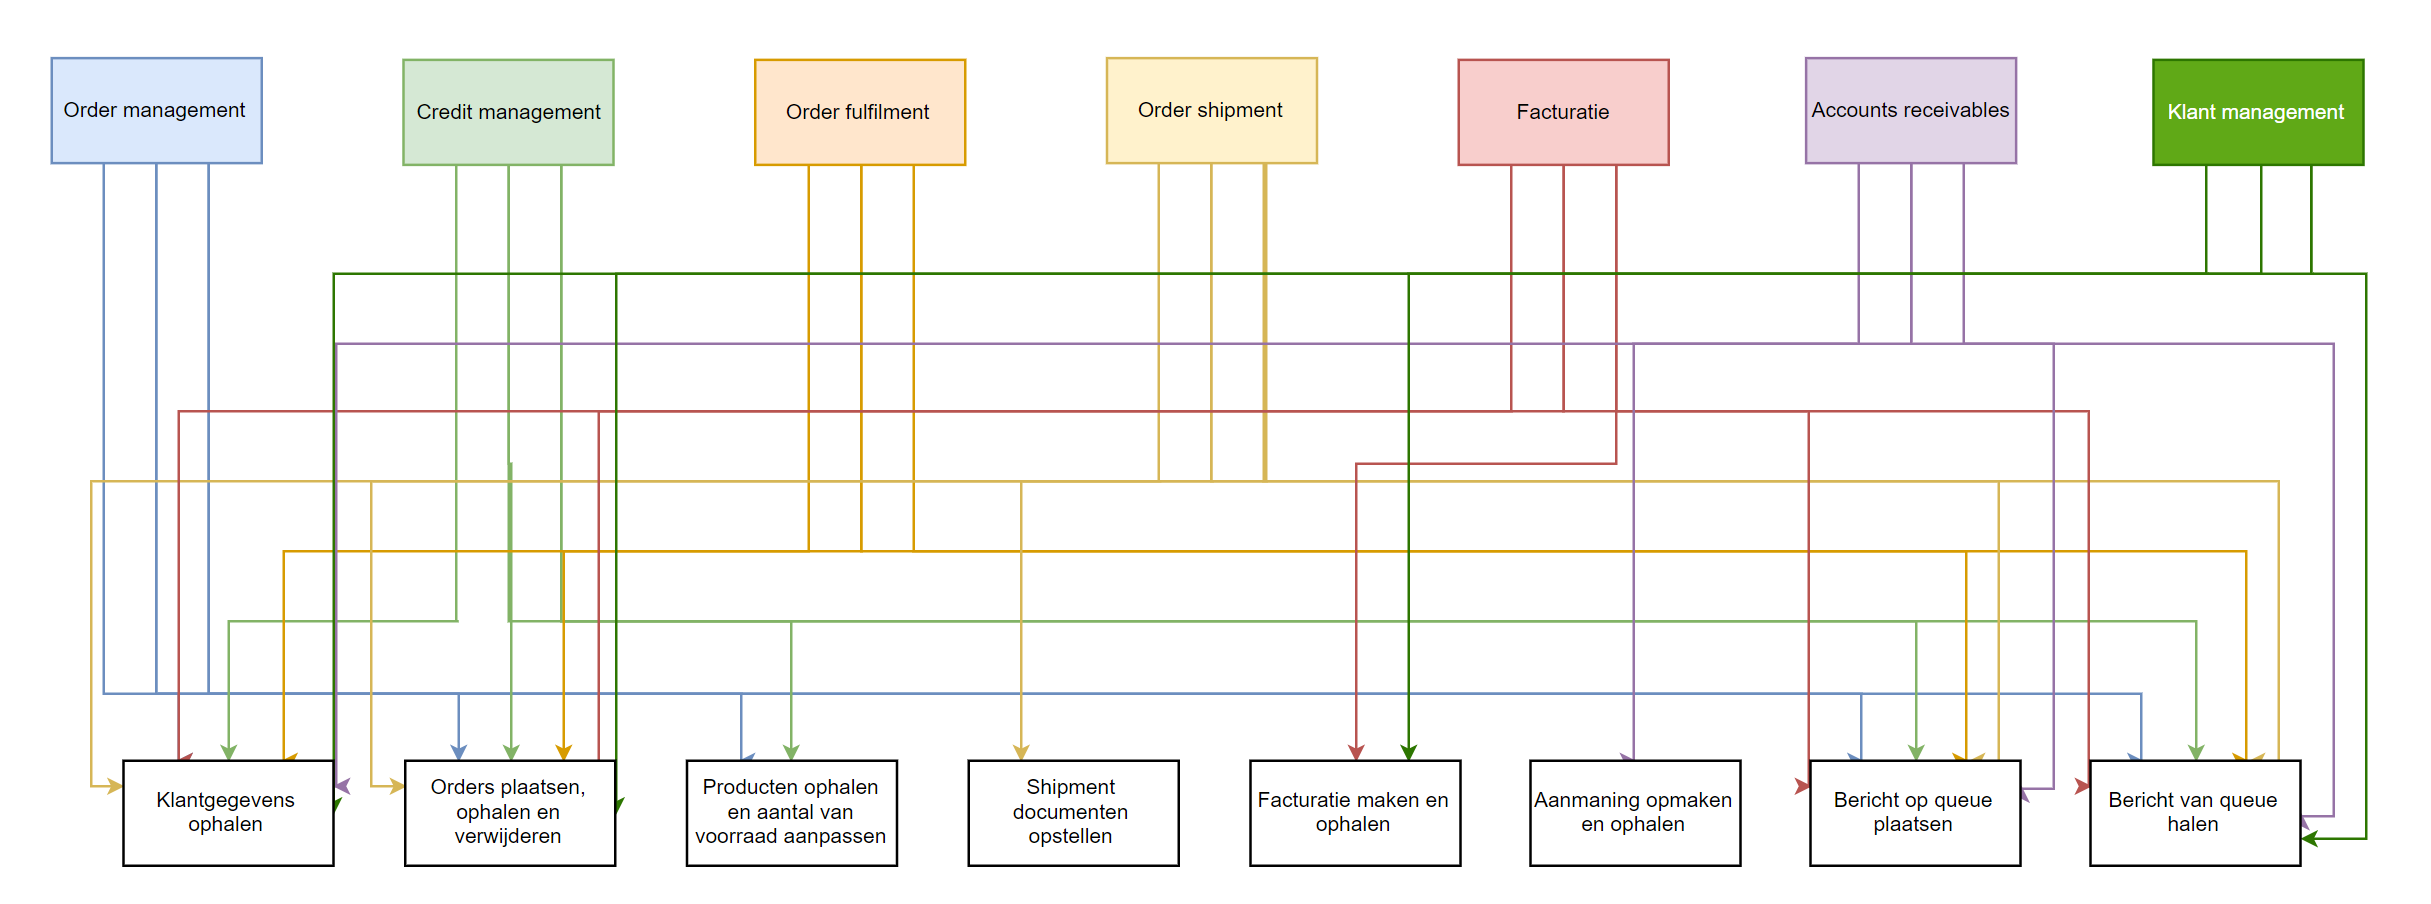
\includegraphics[width=15cm]{schema_microservices.png}
	\caption{Welk onderdeel, welke microservices aanspreekt.}
	\centering
\end{figure}

\subsubsection{Order management}
\begin{figure}[h]
	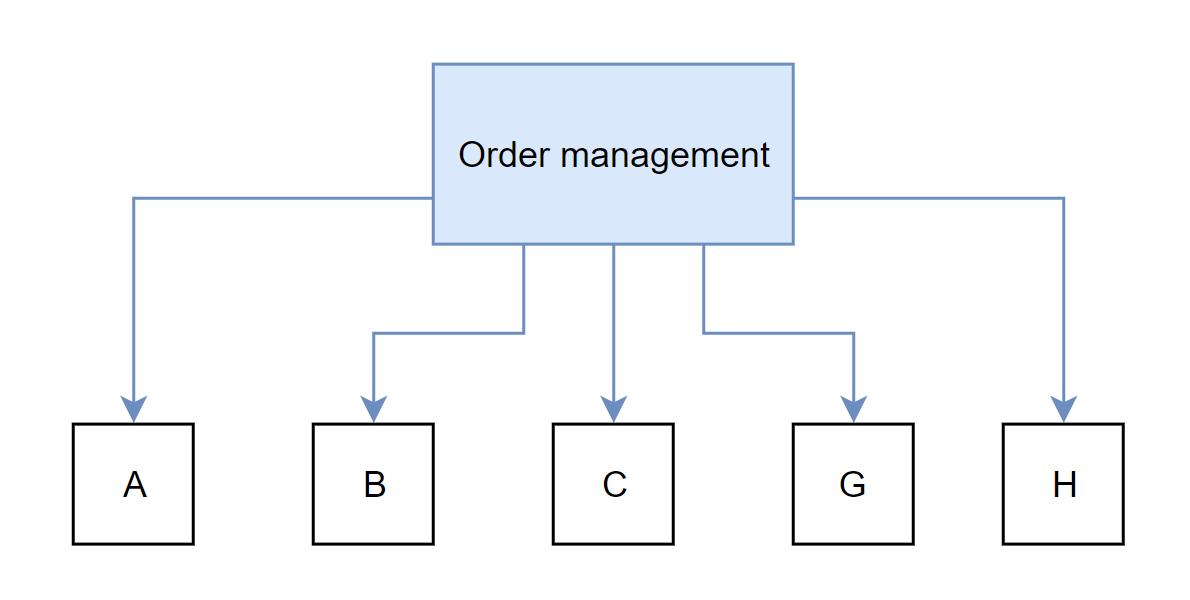
\includegraphics[width=5cm]{ordermanagement.png}
	\caption{Order management communiceert met volgende microservices.}
	\centering
\end{figure}
Order management communiceert met volgende microservices:
\begin{itemize}
	\item Klantgegevens ophalen.
	\item Orders plaatsen, ophalen en verwijderen.
	\item Producten ophalen en het aantal van de voorraad aanpassen.
	\item Bericht plaatsen op queue.
	\item Bericht van queue halen.
\end{itemize}
Een klant plaatst een order op het platform van het bedrijf. De gegevens van de klant worden opgehaald en gelinkt aan het nieuw gecreëerde order. Eens die twee taken zijn afgerond, wordt het bericht op de queue geplaatst van credit management.

\subsubsection{Credit management}
\begin{figure}[h]
	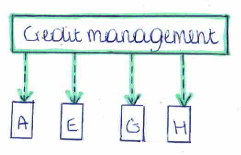
\includegraphics[width=5cm]{creditmanagement.png}
	\caption{Credit management communiceert met volgende microservices.}
	\centering
\end{figure}
Credit management communiceert met volgende microservices:
\begin{itemize}
	\item Klantgegevens ophalen.
	\item Orders ophalen, plaatsen en verwijderen.
	\item Facturatie maken en ophalen.
	\item Bericht plaatsen op queue.
	\item Bericht van queue halen.
\end{itemize}
Eerst wordt het bericht dat door order management op de queue geplaatst werd, opgehaald. Dan is er een klantnummer en een ordernummer. Bij credit management kijkt of de klant een goed betaalgedrag heeft. Staat de klant gekend als wanbetaler dan naar het order gegaan om de plaatsing van het order af te keuren. In andere gevallen krijgt de order een goedkeuring en wordt het ordernummer geplaatst op de queue van order fullfilment. Dan zit de taak van credit management erop.

\subsubsection{Order fullfilment}
\begin{figure}[h]
	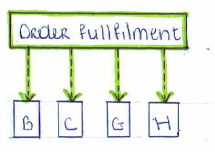
\includegraphics[width=5cm]{orderfullfilment.png}
	\caption{Order fullfilment communiceert met volgende microservices.}
	\centering
\end{figure}
Order fullfilment communiceert met volgende microservices:
\begin{itemize}
	\item Orders ophalen, plaatsen en verwijderen.
	\item Producten ophalen en het aantal in de voorraad aanpassen.
	\item Bericht plaatsen op queue.
	\item Bericht van queue halen.
\end{itemize}
Bij order fullfilment staat er een ordernummer op de queue. Die wordt opgehaald en aan de hand van het ordernummer, weet men welke goederen er uit het magazijn moeten gehaald worden. Voor alle goederen moet het aantal in de voorraad aangepast worden. Eens het order compleet is, wordt het ordernummer op de queue van order shipment geplaatst.

\subsubsection{Order shipment}
\begin{figure}[h]
	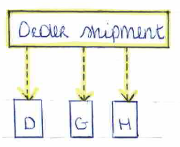
\includegraphics[width=5cm]{ordershipment.png}
	\caption{Order shipment communiceert met volgende microservices.}
	\centering
\end{figure}
Order shipment communiceert met volgende microservices:
\begin{itemize}
	\item Orders ophalen, plaatsen en verwijderen.
	\item Klantgegevens ophalen.
	\item Shipment document opstellen.
	\item Bericht plaatsen op queue.
	\item Bericht van queue halen.
\end{itemize}
Order shipment krijgt het ordernummer binnen via zijn queue. Het order wordt bekeken en de klant gegevens worden opgehaald aan de hand van het gekoppelde klantnummer aan het order. Eens het order shipment document is opgesteld en alle goederen klaar zijn voor vertrek, wordt het ordernummer geplaatst op de queue van facturatie.

\subsubsection{Facturatie}
\begin{figure}[h]
	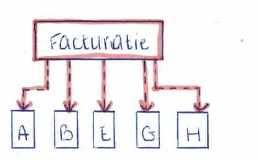
\includegraphics[width=5cm]{facturatie.png}
	\caption{Facturatie communiceert met volgende microservices.}
	\centering
\end{figure}
Facturatie communiceert met volgende microservices:
\begin{itemize}
	\item Klantgegevens ophalen.
	\item Orders ophalen, plaatsen en verwijderen.
	\item Facturatie maken en ophalen.
	\item Bericht plaatsen op queue.
	\item Bericht van queue halen.
\end{itemize}
Eens het ordernummer opgehaald is van de queue, wordt alle nodig info opgehaald om de factuur op te maken. De nodige gegevens zijn klantgegevens en het order. Eens de factuur opgemaakt is, wordt het factuur nummer geplaatst op de queue van account receivables.

\subsubsection{Accounts receivables}
\begin{figure}[h]
	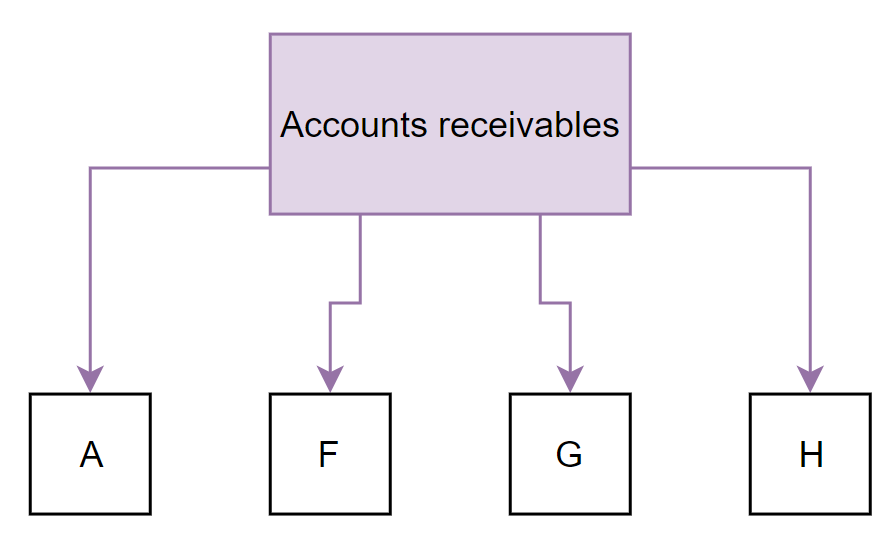
\includegraphics[width=5cm]{accountreceivables.png}
	\caption{Accounts receivables communiceert met volgende microservices.}
	\centering
\end{figure}
Accounts receivable gaat na of de betaling wel goed wordt afgerond. Om dit te kunnen, worden volgende microservices aangesproken:
\begin{itemize}
	\item Klantgegevens ophalen.
	\item Facturatie maken en ophalen.
	\item Bericht plaatsen op queue.
	\item Bericht van queue halen.
\end{itemize}

\subsubsection{Klant management}
\begin{figure}[h]
	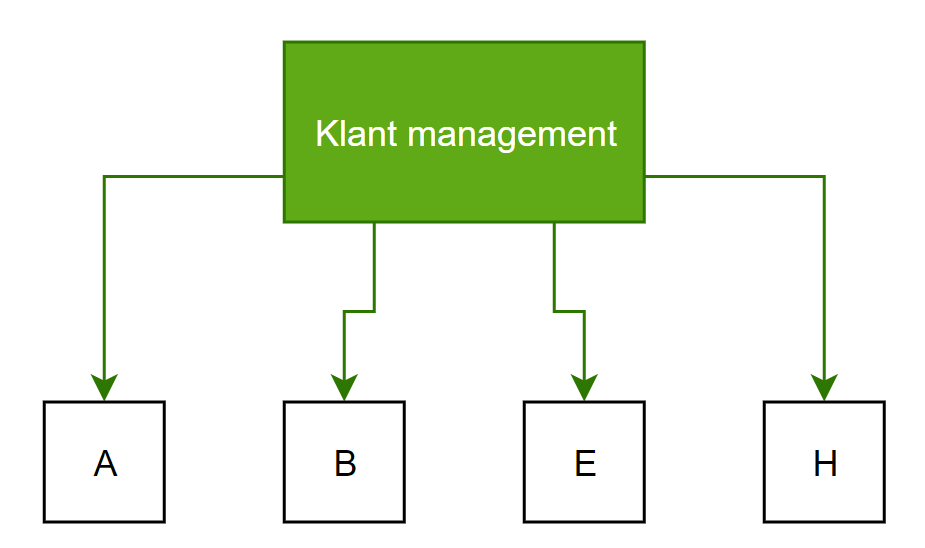
\includegraphics[width=5cm]{klantmanagement.png}
	\caption{Klant management communiceert met volgende microservices.}
	\centering
\end{figure}
Klant management staat in voor het contact met de klant. Dit deel gebruikt volgende microservices:
\begin{itemize}
	\item Klantgegevens ophalen.
	\item Orders ophalen, plaatsen en verwijderen.
	\item Facturatie maken en ophalen.
	\item Bericht van queue halen.
\end{itemize}
Als een van de vorige onderdelen een bericht plaatst op de queue, zal die verwerkt worden en de nodige info wordt opgehaald.

\subsection{De volgende stappen: Het toevoegen van API, logging en authenticatie en authorisatie}
\subsubsection{Logging}
Logging kan toegepast worden door nog een extra microservice te ontwikkelen. Hiernaar kunnen de andere microservices hun logs posten. Hier zal niet verder op worden ingegaan. 

\subsubsection{API gateway}
Een API gateway wordt toegevoegd om ervoor te zorgen dat de architctuur niet openbaar is voor iedereen. Er is één aanspreekpunt en die regelt de rest van de communicatie.
De API communiceert in dit geval enkel met order management. De API geeft alle nodige informatie door en order management schrijft deze weg naar de datastore en naar de databank.
\begin{figure}[h]
	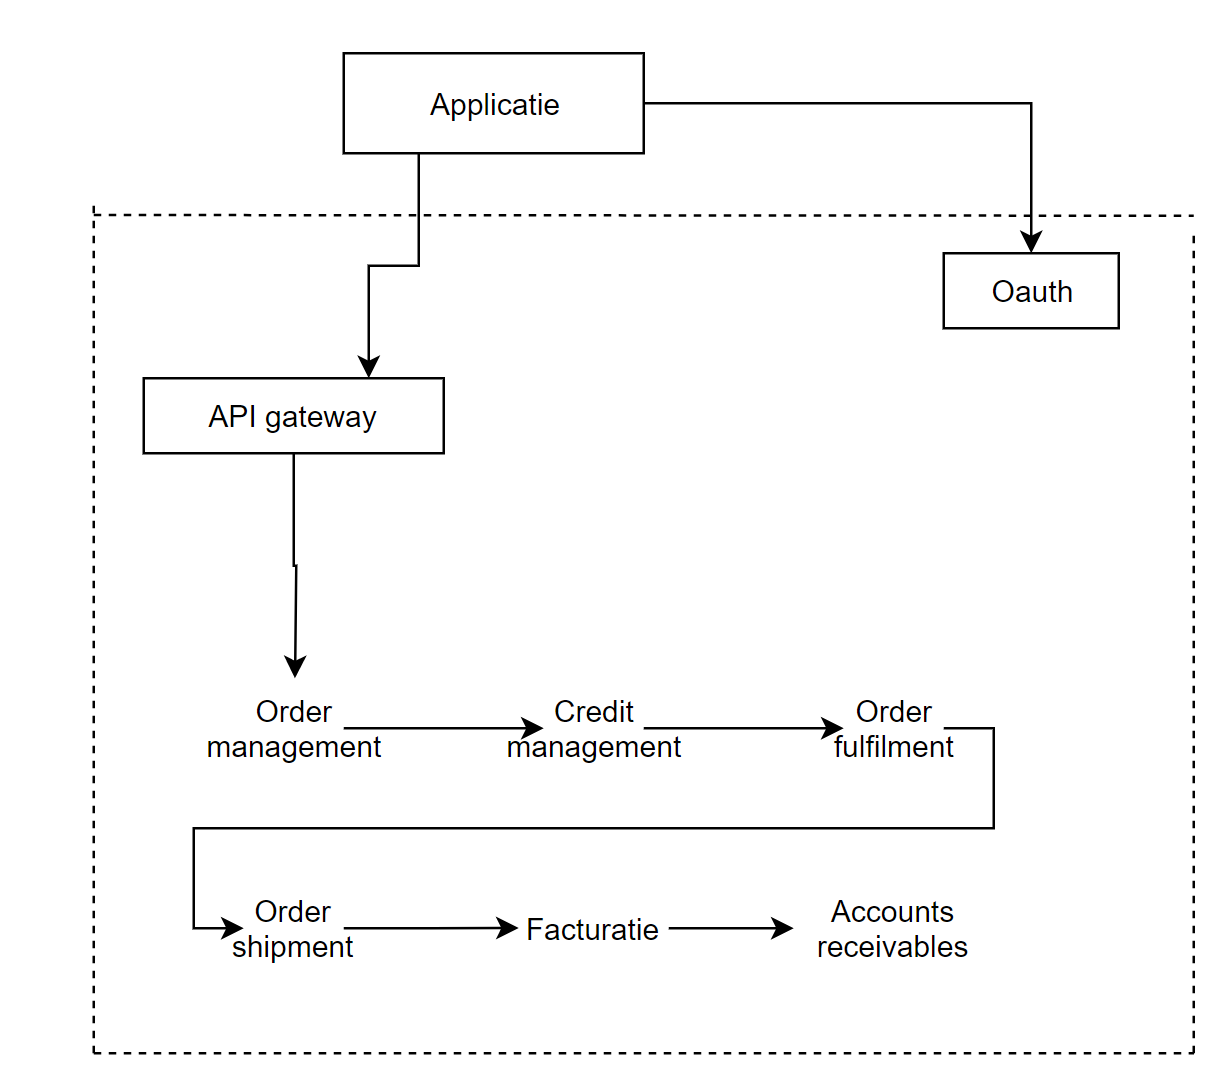
\includegraphics[width=10cm]{apiSchema.png}
	\caption{Vereenvoudigd schema.}
	\centering
\end{figure}

\subsubsection{Authenticatie en autorisatie}
Onder het hoofdstuk 'stand van zaken', is een vergelijking te vinden over authenticatie. Uit die vergelijking, is de keuzen API gekozen als authenticatie. Binnen API zijn er verschillende opties, die worden ook overlopen in het vorige hoofdstuk. Er is gekozen voor OAuth omdat dit de meest bekende en gebruikte versie is.

De gebruiker moet gekend zijn voordat die een order kan plaatsen. De authenticatie van de gebruiker gebeurt vooraf. Er is een aparte micrservice voor authenticatie. Hier wordt niet dieper op in gegaan.
Op afbeelding 3.12 is wel een mogelijke plaatsing zichtbaar.




% Voeg hier je eigen hoofdstukken toe die de ``corpus'' van je bachelorproef
% vormen. De structuur en titels hangen af van je eigen onderzoek. Je kan bv.
% elke fase in je onderzoek in een apart hoofdstuk bespreken.

%\input{...}
%\input{...}
%...

%%=============================================================================
%% Conclusie
%%=============================================================================

\chapter{Conclusie}
\label{ch:conclusie}

% TODO: Trek een duidelijke conclusie, in de vorm van een antwoord op de
% onderzoeksvra(a)g(en). Wat was jouw bijdrage aan het onderzoeksdomein en
% hoe biedt dit meerwaarde aan het vakgebied/doelgroep? 
% Reflecteer kritisch over het resultaat. In Engelse teksten wordt deze sectie
% ``Discussion'' genoemd. Had je deze uitkomst verwacht? Zijn er zaken die nog
% niet duidelijk zijn?
% Heeft het onderzoek geleid tot nieuwe vragen die uitnodigen tot verder 
%onderzoek?

De conclusie van deze theoretische studie is dat aan de hand van microservices, het order-to-cash proces geautomatiseerd kan worden. 

Microservice kan in meerdere contexten voor komen. Binnen elke context zal er meer verkaring nodig zijn.

Authorisatie en authenticatie kan toe gepast worden op verscheidene manieren. Naargelang de noden van de applicatie kan de wijze van deze verschillen. 

Bescherming kan op verschillende manieren toegepast worden. Hier moet er aan grondige research gedaan worden om te beslissen welke manier de beste is. 

Microservice is een architectuur en ideologie waarin logica en de requirements, die te vinden zijn bij een monolithic, terugkomen. Dit heeft invloed op de overschakeling naar microservices. Deze manier van implementatie moet aangepast worden bij het gebruik van microservices. Dat kan een obstakel zijn. Er wordt een andere manier van denken en organiseren gevraagd binnen een de IT-afdeling. De teams worden hervormd. Een team bevat niet meer de kennis van de volledige architectuur., enkel over de microservice waaraan zij werken. 

Een ander punt dat aan bodt komt, is de veranderingen die gebeuren. Die worden in volgende opsomming weergegeven:
\begin{itemize}
	\item Heeft deze applicatie nood aan een microservice architectuur?
	\item De databank structuur moet herbekeken worden.
	\item Het volledige proces herbekijken.
	\item De manier van communiceren tussen de verschillende onderdelen moet worden onderzocht.
	\item Welke manier van authenticatie en authorisatie gaat men gebruiken?
	\item Welke manier van bescherming kan er toegepast worden?
	\item Moeten we de teams herstructureren?
\end{itemize}

De veranderingen die werden toegepast aan het OTC-proces zijn gelijklopend met de opsomming hierboven. 
Door de uitwerking, is het duidelijk geworden hoe microservices meerdere keren gebruikt kunnen worden. Als men kijkt naar de microservice 'klantgegevens ophalen', ziet men dat deze meermaals gebruikt wordt binnen de architectuur. 

Ten slotte kan er geconcludeerd worden dat:
\begin{itemize}
	\item Microservices een brede term is en kan voorkomen in verschillende contexten.
	\item Een microservice architectuur niet altijd nodig is.
	\item Microservices kunnen een OTC proces automatiseren.
	\item Microservices zorgen ervoor dat elk onderdeel van het proces apart kan functioneren.
\end{itemize}

Zelf heb ik ondervonden dat het aanpassen van een monolithic niet eenvoudig is. De monolithic architectuur zit ingebakken in het informatica landschap. De manier van omgang met microservices, kan vergeleken worden met die van Agile. De Agile methode moest in eerste instatie zijn toegevoegde waarde op een project bewijzen. Dan pas zijn projectmanagers deze ook gaan gebruiken. Microservices zal eerst zijn voordeel moeten bewijzen ten opzichte van monolithic om een statement te kunnen maken.





%%=============================================================================
%% Bijlagen
%%=============================================================================

\appendix
\renewcommand{\chaptername}{Appendix}

%%---------- Onderzoeksvoorstel -----------------------------------------------

\chapter{Onderzoeksvoorstel}

Het onderwerp van deze bachelorproef is gebaseerd op een onderzoeksvoorstel dat vooraf werd beoordeeld door de promotor. Dat voorstel is opgenomen in deze bijlage.

% Verwijzing naar het bestand met de inhoud van het onderzoeksvoorstel
%---------- Inleiding ---------------------------------------------------------

\section{Introductie} % The \section*{} command stops section numbering
\label{sec:introductie}

Hoe Microservice integration patterns een order to cash proces in SAP beinvloedt. Dit onderwerp werd gekozen omdat deze nieuwe technology een interessante invloed kan hebben op de order-to-cash proces. Dit is een manier om een proces robuuster te maken. In de meeste software wordt gebruik gemaakt van één grote databank of meerdere databanken die in staan zijn om meerde services te voorzien van data. Bij microservice integration patterns wordt voor elke service een aparte databank opgesteld. Dit is maar een klein deeltje van een microservice. De microservices moeten voldoen aan business requirements. SAP zelf heeft ook al veel ondernomen omtrend microservices. Eén van hun oplossingen is Kyma. Maar de belangrijkste vraag is namelijk: Hoe microservice integration patterns een order-to-cash in SAP beïnvloedt. Deze bachelorproef zal voor het grootste deel een theoretische vergelijking zijn. Omdat deze studie als bachelorproef dient, is er maar beperkte tijd en resources om een onderzoek te doen. 

%---------- Stand van zaken ---------------------------------------------------

\section{Literatuurstudie}
\label{sec:state-of-the-art}

Over het onderwerp "Microservice Integration Patterns on Order-to-Cash proces in SAP", zijn er nauwelijks thesissen te vinden. De meeste informatie komt uit artikels die meer uitleg geven over microservices en artikels met een uitgebreide beschrijving over wat order-to-cash inhoudt.
Voor wie denkt dat microservices iets nieuws is, zit er een beetje naast. Grote bedrijven zoals Netflix, Twitter, Amazon en facebook maken al gebruik van deze technologie. ~\cite{CiberBlog2018}

\subsection{Wat zijn microservices?}
Het bouwen van aparte functies/modules met hun eigen interface en methoden. Deze manier van werken is in het voordeel van Agile. Bij Agile wordt er gewerkt met deeltjes software opleveren en opgeleverde software, daar wordt er zo goed als niks meer aan veranderd. Microservices worden onderverdeeld aan de hand van business requirements. Deels zorgen microservices ervoor dat er beter moet worden samengewerkt met de business.

\subsection{Waarom microservices gebruiken} 
In het artikel van ~\cite{Gunaratne2018} werd besproken hoe je een microservice werkt. En waarom deze gebruikt worden. Volgens dit artikel zijn microservices een goede, nieuwe techniek die op lange termijn huidige SOA's kan vervangen. 

~\cite{Atrash2018} beschrijft waarom je deze techniek kunt gebruiken, in de plaats van de kleinere SOA-services. Ook hier wordt verwezen naar de belangrijkheid van de requirements van de business. Door de grootte van deze services, is er de mogelijkheid om te caching. 

~\cite{devoteam2018} legt uit waarom microservices een kleine-SOA is. Een microservice omvat bepaalde, aanvullende, concepten omliggend deze 'kleinere services' en dit is waar ze beginnen met aantonen van de verschillen.

Is de integratie van microservices wel mogelijk? Deze vraag beantwoordt door ~\cite{VanBart2018}. Software wordt meestal nog geimplementeerd in de 3-tiers manier. Ook wel monolithic genoemd. De applicatie is uit een alleenstaande unit gemaakt. Eén verandering heeft een impact op de volledige applicatie. Is dit dan een geldige reden om voor microservices te kiezen? Dat hangt af van wat je applicatie percies nodig heeft. Niet alle applicaties worden er beter van om een microservice te implementeren. Een microservice  bestaat er uit om op zichzelf te werken. Dit wordt uitgelegd in het volgende deel.

\subsection{Principes voor Microservices Integration}

De principes van microservices integration werden uitgelegd in volgend artikel ~\cite{Aradheye2018}
In het artikel wordt op een duidelijke manier uitgelegd hoe microservices worden gebruikt. Microservices worden het best opgesteld aan de hand van business units. Een microservice wordt benaderd vanuit de business requirements. Deze hebben, volgens dit artikel, een betere performantie dan de huidig gebruikte techniek. Microservices worden opgedeeld in verschillende klasses. Bijvoorbeeld:
\begin{itemize}
	\item één voor klantendata
	\item één voor bestellingen
	\item één voor "wil-ik" lijsten
\end{itemize}

De belangrijkste eigenschappen van microservices zijn:
\begin{itemize}
	\item Microservice bestaat uit meerdere componenten
	\item Gemaakt voor de business
	\item Microservice maakt gebruik van simpele routing
	\item Een microservice is gedecentraliseerd
	\item Een microservice werkt zelfstandig
\end{itemize}

\subsection{Order-to-cash in SAP}
Order-to-cash is een van de vele processen in SAP die vast gelegd zijn. Dit proces legt uit hoe men van een bestelling naar de inning van het geld gaat. Er zijn verschillende versies van hoe het proces gaat. Volgens ~\cite{Akthar2018} verloopt het proces als volgt: er wordt een order geplaatst dan wordt die bestelling geleverd, daarna wordt er een factuur opgesteld en als laatste wordt het geld geind. Het proces op zich is niet ingewikkeld. ~\cite{OpenSap2018} geeft veel meer uitleg over wat er achter de schermen gebeurd. Bij dit proces wordt de financiële kant van SAP aangesproken, ook de verkoop en distributie alsook de stock worden aangesproken. Een gedetailleerder proces houdt in dat er een sales order gemaakt wordt. Dan wordt de stock bekeken. Afhankelijk van de beschikbaarheid van de goederen kan er een levering gepland worden. Zijn de goederen beschikbaar, dan kan er na de planning van de levering, effectief geleverd worden. Als volgt wordt er een factuur opgemaakt. Als laatste komt dan het betalingsproces. 

\subsection{Kyma}
Kyma is een open-source project van SAP. Het is vooral gebaseerd op Kubernetes. Op deze manier kan je oplossingen in de Cloud maken. Kyma is special omdat zij zo goed als alle oplossingen op één plek hebben. Zij hebben een application connector. Kyma is serverless. Ze maken service management eenvoudiger. ~\cite{Kyma2019}
Volgens het artikel van ~\cite{Semerdzhiev2018} is er meer nood aan openheid en een modernere architectuur. Dat is ook de reden waarom Kyma een open source project is. Kyma ondersteund container-based werken (zoals docker) alsook cloud-native apps. 

% Voor literatuurverwijzingen zijn er twee belangrijke commando's:
% \autocite{KEY} => (Auteur, jaartal) Gebruik dit als de naam van de auteur
%   geen onderdeel is van de zin.
% \textcite{KEY} => Auteur (jaartal)  Gebruik dit als de auteursnaam wel een
%   functie heeft in de zin (bv. ``Uit onderzoek door Doll & Hill (1954) bleek
%   ...'')

%---------- Methodologie ------------------------------------------------------
\section{Methodologie}
\label{sec:methodologie}
In dit werk gaan we onderzoeken op welke manier microservices een invloed zou kunnen hebben op een order-to-cash proces in SAP. De services die ze nu gebruiken vergelijken met microservices. Kunnen microservices de werking van SAP versnellen en performanter maken bij fouten?
Eerst willen we het volledige order-to-cash proces verstaan. Dan gaan we gaan onderzoeken welke verschillende mogelijkheden er zijn in verband met microservices. Kyma, PaaS.io of zijn er nog andere die een grote rol kunnen spelen. Ook moet er gekeken worden welke manier van communiceren tussen de microservices het beste is. Voor dit onderzoek zal er veel literatuur studie gedaan worden. 


%---------- Verwachte resultaten ----------------------------------------------
\section{Verwachte resultaten}
\label{sec:verwachte_resultaten}
Naar de al gelezen literatuur kijkende, zou Kyma eigenlijk de beste oplossing moeten zijn. Deze is namelijk zelf afkomstig van SAP. Dit zou een goede oplossing moeten zijn. Maar zijn microservices wel haalbaar in een order-to-cash proces in SAP. Eerst zal dit duidelijk moeten worden vooraleer we gaan kijken naar welke microservice de best mogelijk noden opvult. 


%---------- Verwachte conclusies ----------------------------------------------
\section{Verwachte conclusies}
\label{sec:verwachte_conclusies}

De conclusie die we uit dit onderzoek  kunnen trekken: microservices integration patterns zijn voordeliger en gebruiksvriendelijker dan het huidige systeem is voor de mensen die de software gaan gebruiken. Bij fouten aan een service, zal het platform nog beschikbaar zijn. Het risico is wel dat door de relatief nieuwe techniek, er enkele dingen niet zullen lopen zoals we zouden willen. Het is mogelijk dat we maar tot een gedeeltelijke conclusie komen.



%%---------- Andere bijlagen --------------------------------------------------
% TODO: Voeg hier eventuele andere bijlagen toe
%\input{...}

%%---------- Referentielijst --------------------------------------------------

\printbibliography[heading=bibintoc]

\end{document}
